\section{Diskussion \& Ausblick}
Bei dem Vergleich von \textsc{MiniDogNN} mit \textsc{PreBigDogNN},
zeigt sich deutlich, welchen Einfluss die Featureanzahl auf die Genauigkeit hat.
DDesweiteren zeigt sich bei \textsc{MiniDoggNN}-Architektur
für $120$ Rassen, dass die Anzahl der Neuronen pro Lage eine geringe Anzahl an
Features scheinbar nicht ausgleichen kann.

Die geringe Genauigkeit des alternative Ansatzes ist vermutlich auf die
geringe Bildgröße von $96\times96$ zurückzuführen.
Ein Hyperparamter der sich auch auf die Genauigkeit der vortrainierten Modelle
auswirken kann. Diese Korrelation lässt sich auf den Informationsrverlust bei
einer Verkleinerung zurückführen.

Die durchgeführt HPO für das \textsc{MiniDogNN} zeigt, den Einfluss der
Hyperparamter auf ein Modell. Durch eine Vergrößerung
des Parameterraumes oder einer zufälligen Parameterwahl kann eventuell noch e
weiter an Genauigkeit gewonnen werden. Insbesondere sollte eine HPO an
\textsc{PreBigDogNN} durchgeführt werden. Bei dieser wäre der Hyperparamter
der Bildgröße, wie oben besprochen, ein interessanter Parameter. Jedoch verdeutlich
die HPO des RF, dass HPOs im Allgemeinen keine Universallösung sein müssen.

Werden beispielhafte Klassifizierungen der \textsc{MiniDogNN}-Architektur (vgl. Abb. \ref{fig:klasifizierung_MiniDogNN}) betrachtet, werden die Aussagen der Confusionmatrix
(vgl. Abb. \ref{fig:MiniDogNN_Konfusionmatrix}) bestätigt.
\begin{figure}
\centering
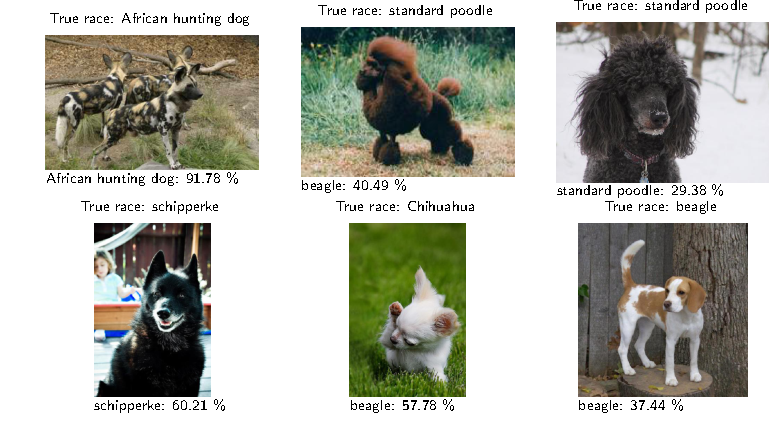
\includegraphics[width = 0.7\textwidth]{../../final_data/MiniNN_n5/visualize_predictions.pdf}
\caption{Beispielhafte Klassifizierung des Testdatensatzes mit \textsc{MiniDogNN}.
        Die Prozentzahl unter jedem Bild gibt die Wahrscheinlichkeit für die Klassenzugehörigkeit an.}
\label{fig:klasifizierung_MiniDogNN}
\end{figure}
In der Konfusionmatrix \ref{fig:MiniDogNN_Konfusionmatrix} hat sich gezeigt, dass
die Rasse \emph{Schipperke} oft mit der Rasse \emph{African Hunting Dog} verwechselt
wird. Dies könnte mit der Ähnlichkeit in der Schnauzenform erklärt werden. Desweiteren
können die Schwierigkeiten mit der \emph{Beagle} und \emph{Chihuahua} Klassifizierung
durch die Fellfarbe erklärt werden. Insbesondere beim kleinen Datensatz kann dies,
auf Grund der geringeren Statistik, eine große Auswirkung haben. Über diesen Ansatz
könnte auch die schlechte Klassifizierung der \emph{Poodle} Rasse erklärt werden.
Die Rassen \emph{Schipperke} und \emph{African Hunting Dog} besitzen wie die
\emph{Poodle} Rasse oftmals dunkles Fell. Das Fell des \emph{Poodles} unterscheidt sich
jedochin der Struktur, was eventuell von dem \textsc{MiniDogNN}-CNN nicht, aber von dem
\textsc{PreDogNN} als Feature festgestellt werden konnte.

An dieser Stelle, muss noch die Reproduzierbarkeit der Ergebnisse beleuchtet werden.
Während des wiederholten Trainings, unter Verwendung der selben Parameter, eines Modells
ergeben sich oftmals unterschiedliche Confusionmatrizen. Die Grundgestalt wie zum Beispiel
die Existenz einer Diagonale bleibt erhalten, jedoch können sich die Nebendiagonalelemente
stark voneinander unterscheiden. Dieser Effekt kann nicht auf die Data Augementation
zurückgeführt werden, da hier ein Seed gesetzt wurde. Wahrscheinlicher ist ein Einfluss
der Grafikarte auf das Trainieren, da intern auch Zufallsoperation durchgeführt werden,
wie in der Quelle \cite{Reproduzierbarkeit} erläutert wird.

Die Motivation für dieses Projekt war es, einen Klassifizier zu erstellen,
der besser ist, als der durchschnittliche TU Dortmund Physikstudierende.
Es lässt sich zusammenfassen, dass lediglich die \textsc{PreBigDogNN}-Architektur
einen Physikstudierenden schlagen würde. In Verbindung mit
der formulierten Hypothese wird deutlich, dass die \textsc{PreBigDogNN}-Architektur
einem Physikstudierenden der TU Dortmund überlegen ist und eventuell als Hilfsmittel
in Betracht gezogen werden sollte.

Abschließend soll noch ein Ausblick über mögliche Verbesserung gegeben werden.
Wie bereits in der Diskussion erwähnt könnte sich die Bildgröße, bis zu einer
Art Sättigung, signifikant auf die Genauigkeit auswirken. Momentan ist das
Framework hierdurch die Beschaffenheit von \textsc{numpy.arrays} beschränkt.
Jedoch könnte die Verwendung von \textsc{python} \textsc{dictonaries} eine Lösung sein,
da einzelne Einträge nicht die gleiche Shape benötigen. Darüberhinaus sollte mittels
HPO die optimalen Hyperparameter für die vortrainierten Modelle ermittelten werden.
Die Performance der vortrainierten Modelle könnte weiterhin auch durch die Anpassung
des FCN verbessert werden. Eine letzte Möglichkeit die Genauigkeit zu erhöhen,
wäre den Datensatz eigenständig zu erweitern.

\newpage
